\documentclass[a0,final]{a0poster}
%%%Load packages
\usepackage{multicol} 			%3-column layout
\usepackage[left=2cm,right=2cm,bottom=1cm,top=0cm]{geometry}			%Reset margins
\usepackage{mathpazo}			%Load palatino font & pazo math
\usepackage{color}				%Needed for colour boxes & coloured text
\usepackage{hyperref}
\usepackage{graphicx}
\graphicspath{{img/}}
\usepackage{minted}
\usepackage{csquotes}

%%%Define colours and lengths
\definecolor{headingcol}{rgb}{1,1,1}			%Colour of main title
\definecolor{boxcol}{rgb}{0.0,0.2,0.4}		%Edge-colour of box and top banner
\fboxsep=1cm							%Padding between box and text
\setlength{\columnsep}{2cm}				%Set spacing between columns

%%%Format title
\makeatletter							%Needed to include code in main file
\renewcommand\@maketitle{%
\null									%Sets position marker
{
\color{headingcol}\sffamily\VERYHuge		%Set title font and colour
\@title \par}%
\vskip 0.6em%
{
\color{white}\sffamily\large				%Set author font and colour
\lineskip .5em%
\begin{tabular}[t]{l}%
\@author
\end{tabular}\par}%
\vskip 1cm
\par
}
\makeatother

\title{Assembling accentual verse with Twitter and the NLTK}

\author{
Stephen Krewson\\
Department of English Language and Literature, Department of Computer Science\\
\url{stephen.krewson@yale.edu}
}

\begin{document}

\hspace{-3cm}								%Align with edge of page, not margin
\colorbox{boxcol}{							%Coloured banner across top
\begin{minipage}{1189mm}					%Minipage for title contents
\maketitle
\end{minipage}}
\vspace{1cm}

\begin{multicols}{3}							%Use 3-column layout
\raggedcolumns							%Don't stretch contents vertically

%%%Column1
\section*{Introduction}
This project is an outgrowth of my very first programming project, which dates back to my time in LING 327 (627), ``Language and Computation.'' That course--the first elective I took during my PhD program--was taught using Python and I wanted to take the techniques I was learning and use them for creative writing (my undergraduate major).\\
\\
Around that time I also discovered \url{@pentametron}, an alias under which Ranjit Bhatnagar collected tweets that could scan as iambic pentameter and then patched them together into a sonnets. Here's an example. Pentametron has used a few different rhyme schemes; in this case, it's ABAB CDCD EFEF GG for a pretty straightforward case of Shakespearean.\\

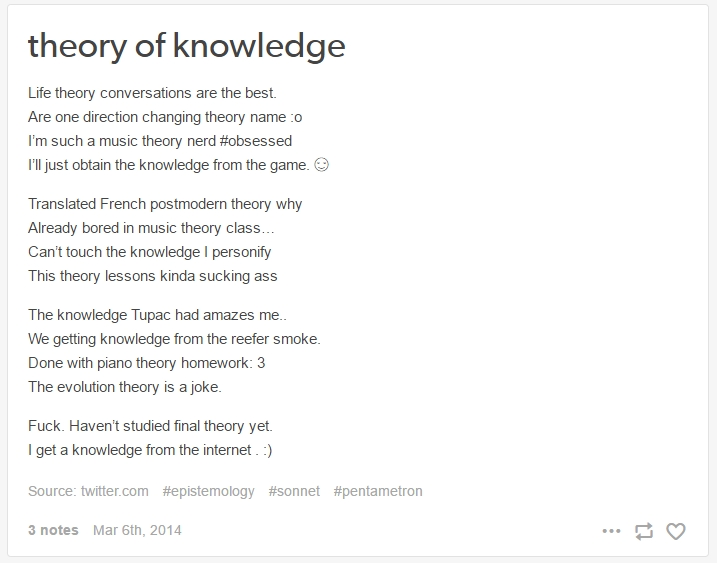
\includegraphics{tweet1.jpg}\\
\\
I would later find out that Bhatnagar's program was written in PHP and used Carnegie Mellon University's Pronouncing Dictionary (\url{http://www.speech.cs.cmu.edu/cgi-bin/cmudict}). But when I set out to reverse-engineer some of Pentametron's functionality, all I knew was Python and the Natural Language Toolkit library (NLTK). So I set out to make a Twitter poetry generator for an art installation conceived by XS Collaborative, an interdisciplinary group of Yale grad students who took over several abandoned storefronts in 2013.


\section*{Twitter API}
Of course, the first thing I needed to wire up was Twitter, which allows users to sign up for a developer account (\url{https://dev.twitter.com/}) and then generate tokens for authenticating to their API (``application program interface'') and accessing real-time data. Twitter exposes a RESTful public search API that allows multi-parameter HTTP requests like the following.\\

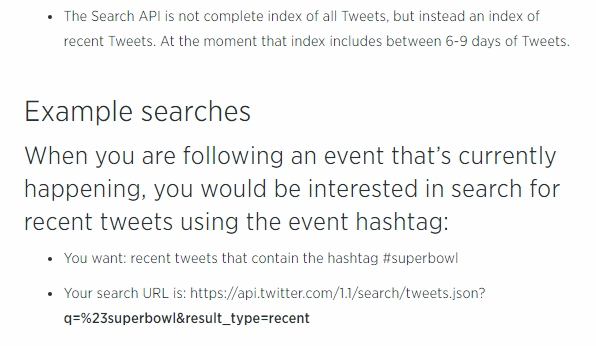
\includegraphics{tweet3.jpg}\\
\\
This GET request will, if successful, return a JSON object from within which we can get to what we want, which is simply the raw text of the tweet. Note that Twitter tries to give you relevant tweets from the past week or so, not necessarily all the tweets or the most recent tweets that contain your search parameter. Here's a snapshot of my XS program, displaying a search of the word ``lexicon,'' with some random text from Project Gutenberg mashed in!\\


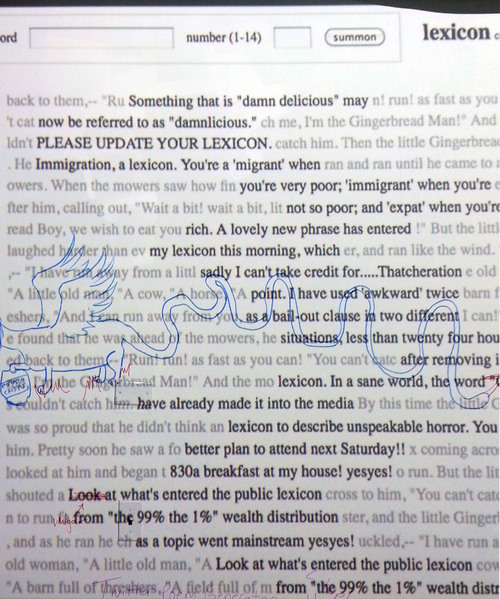
\includegraphics{tweet4.jpg}\\
\\

\section*{Python Libraries}
Thankfully, Python's extensive community means there are third-party libraries that ``wrap'' the HTTP requests that Twitter has promised to support. It was no problem at all to start up the ``twitter'' package at \url{https://pypi.python.org/pypi/twitter}. Here is my code for authenticating with my app credentials and then making a sample request to the search endpoint.\\

\begin{minted}[linenos, frame=lines]{python}
import twitter

from config import twitter_keys

api = twitter.Api(consumer_key=twitter_keys['consumer_key'],
	consumer_secret=twitter_keys['consumer_secret'],
	access_token_key=twitter_keys['access_token_key'],
	access_token_secret=twitter_keys['access_token_secret']
)

results = api.GetSearch('your_search_term')
\end{minted}
%\columnbreak
This gets me an array of tweets (represented as strings) that are now ready to be cleaned up (I get rid of RT's and mentions of \url{@users}, but I don't try to filter emoji or ASII art!) and sent to the NLTK (\url{http://www.nltk.org/install.html}).\\
\\
Turns out, NLTK makes it very easy (by calling that same CMU Pronouncing Dictionary) to scan for lexical stress patterns. For instance, if I process a word with the function ``stripWord'' (below), NLTK can break the word down into one of 39 phonemes and then tell me if it has a stress value of 0, 1, or 2. Only vowels carry stress. And we can only find out stress values for words in the dictionary (~134,00 words). So I have to use some heuristics, such as guessing that unknown words contain about one stress.\\
\\
What does this have to do with poetry? Well, my code does some hand-wave-y things to sculpt the twitter text into ``lines'' of four stresses each. Usually. And it then groups these lines into quatrains. The four-stress model is a nod to the accentual verse tradition in English that dates back to the days of \emph{Beowulf}. The Wikipedia-level explanation of how accentual verse works today specifies (1) four stresses per line, (2) a pause in the middle of the line, (3) some kind of alliterative pattern governing the stressed syllables.\\
\\
But as Ian Cornelius points out, the attempt to pin down accentual verse and identify it with English-ness has a specific ideological history and in its scientific pretensions is subject to structural revolution.

\begin{displayquote} 
[It] is instructive to take one last look at the accentual paradigm, which originated as an effort to theorize meter as a direct, unmediated expression of language. Stress accent was what English could justly claim as its own and this, as the language’s inner genius, was the truth expressed in its meter. Thus stated, the accentual paradigm is a recognizably nineteenth-century formulation, exhibiting the structures of thought characteristic of that period: the inner natures of things may be ontologically withdrawn, but the objects given to us in experience are nevertheless related to those inner natures as their expression. In an effort to grasp that expression in its pure form, scholars of the early nineteenth century rejected the normative force of Greco-Roman metrics and attempted to comprehend all English verse, as such, under a uniform principle of accentual rhythm. They attempted to bracket, as inessential, both the immanent vagaries of history and the spectral exteriority of norms. Yet it remains the case that metrical systems are inherently normative and that history is inherently digressive. There is a constitutive gap between linguistic givens and metrical systems, and hence always more than one way of correlating language to meter.\cite[481]{10.5406/jenglgermphil.114.4.0459}
\end{displayquote}

I only hope that some ``inner genius'' may animate the riot of Internet language that passes through the metrically-agnostic and unfeeling branches of my code today! The instability of prosody is here a feature, not a bug.

\begin{minted}[linenos, frame=lines]{python}
import nltk

lexicon = nltk.corpus.cmudict.dict()

def stripWord(word):
    """Returns tuple of stripped word, lexical stress count"""
    stress = 0
    word = HTMLParser.HTMLParser().unescape(word)
    stripped = word.lower().translate(string.maketrans('',''), string.punctuation)
    # Regex filters out hashtags, URLs
    if not re.match(r'\"*[@#]|http|RT', word):
        if stripped in lexicon:
            for j in ''.join(lexicon[stripped][0]):
                if j in ('1', '2'): # 1=primary, 2=secondary stress
                    stress += 1
            return word.encode('utf-8'), stress
        else: # Unknown words approximated as 1 total stress
            return word.encode('utf-8'), 1
\end{minted}
%\columnbreak

\section*{Coda}
My code is available on GitHub. Use the following series of commands, where ``hippo'' is just an example search term and 14 is the number of tweets to request from the Twitter API. Two things to watch out for: (1) this code is old and thus only runs on Python 2.7. Python 3 will not work. (2) You'll need to put your own API credentials into a Python dictionary object in a file called \url{config.py} in the top-level directory.\\

\begin{minted}[frame=lines]{bash}
git clone https://github.com/StephenKrewson/twitter-poetry.git
cd twitter-poetry
python poem_builder.py hippo 14
\end{minted}

%\nocite*

\bibliographystyle{plain}
\bibliography{halobib}

\end{multicols}
\end{document}